\documentclass[a4paper, 12pt, x11names]{article}

\usepackage{geometry}

\usepackage[T1, T2A]{fontenc}
\usepackage[utf8]{inputenc}
\usepackage[bulgarian]{babel}
\usepackage[normalem]{ulem}

\usepackage{amsmath}

\usepackage{graphicx}
\graphicspath{ {./../images/} }

\usepackage{minted}

\usepackage{tikz}
\usetikzlibrary{er}
\tikzset{multi attribute/.style={attribute, double distance =1.5pt}}
\tikzset{every entity/.style={draw=orange, fill=orange!20}}
\tikzset{every attribute/.style={draw=MediumPurple4, fill=MediumPurple1!20}}
\tikzset{every relationship/.style={draw=Chartreuse4, fill=Chartreuse2!30}}
\newcommand{\key}[1]{\underline{#1}}
\newcommand{\univname}{Софиийски университет "Св. Климент Охридски"\\Факултет по математика и информатика}

\setlength{\parindent}{0mm}

\begin{document}
\begin{titlepage}
\begin{center}
    
\vspace*{.06\textheight}
{\scshape\large \univname\par}\vspace{1.5cm}

{\huge \bfseries{Курсов проект}\par}\vspace{0.7cm}
\textsc{\small по}\\[0.6cm]
\textsc{\Large Бази от данни}\\[0.5cm]
\textsc{\normalsize спец. Информатика, 3 курс, летен семестър,}\\[0.5cm]
\textsc{\normalsize учебна година 2018/19}\\[1.5cm]
\textsc{\Large Тема: Реализация на база от данни за Училище}\\[2cm]

\begin{minipage}[t]{0.4\textwidth}
\begin{flushleft} \large
{\large \today}\\[1cm]
София
\end{flushleft}
\end{minipage}
\begin{minipage}[t]{0.4\textwidth}
\begin{flushright} \large
\emph{Изготвил:}\\[0.5cm]
Иво Алексеев Стратев\\[0.5cm]
Фак. номер: 45342\\[0.2cm]
Група: 3
\end{flushright}
\end{minipage}
\end{center}
\end{titlepage}

\tableofcontents

\pagebreak

\section{Увод (философски възглед)}
В типична база от данни описваща училище се описват същности - учител, ученик, родител.
Въпреки, че те споделят общи характеристики като: собствено име, фамилно, адрес, електронна поща, мобилен и други.
Тези характеристики биха се използвали по различен начин.
Например по коренно различен начин бихме написали електронно писмо до всеки.
По различен начин бихме говорили със всеки и всеки от тях би говорил с другия по различен начин.
Тоест макар да споделят общи характеристики те биха се ползвали по различен начин в рамките на институцията училище.
Наличието на общи характеристики е следствие на социалният елемент.
Поради тази причина в текущата реализация се избягва използването на наследяване (is a) йерархия.
Защото ако имахме общ родител например човек за тези същности, то това би било грешка в дизайна, която отразява реалността,
но не отразява специфичното за областта знание, за липса на еднотипност на общите характеристики.
По същия начин в текущата реализация на база данни се прави ясно разграничение между учебен час и час на класа.
Тоест в текущата реализация е дадено предимство на спецификата на данните,
вместо спазването на по-общото отразяване на действителността.
В рамките на обектно ориентирания подход автора би използвал интерфейс за оказване на наличието на общи характеристики,
които могат да бъдат извлечени, вместо общ родителски клас. С цел подчертаване на ясното разграничване между същностите.
\section{Описание на множествата същности}
\subsection{Teacher}
Описва учител. Всеки учител има id - уникален идентификатор,
first\_name - собствено име, last\_name - фамилно име,
gender - пол, work\_phone - служебен номер на мобилен,
email - служебен адрес на електронна поща и address - личен адрес.
\subsection{Class}
Описва клас в училището. Всеки клас има id - уникален идентификатор,
school\_year - година на класа,
с цел различаване на класовете през годините (например 12 Б клас през 2016 и 12 Б клас прес 2014),
number - номер на класа, letter - буква на класа за отличаване на паралелките,
class\_room - класна стая, в която се провежда часа на класа,
class\_hour - началото на часа на класа, приемаме, че часа на класа винаги е в петък.
\subsection{Course}
Описва предмет в училището. Всеки предмет има id - уникален идентификатор,
на един конкретен клас се води само от един учител,
name - име на предмета, semester - учебен срок на предмета.
\subsection{Program\_entry}
Описва елемент в учебната програма.
Всеки елемент на учебната програма има id - уникален идентификатор,
course - предмет, който се преподава,
day\_of\_week - в кой ден от седмицата се преподава,
room - стая, в която се преподава,
starts - кога започва съответния час, възможно е часовете за започват през различно време,
а не на кръгъл час или на 15/20-та минута от кръглия час ..., hours - продължителност,
брой учебни часове, допускаме преподаване на блокове.
\subsection{Exam}
Описва контролно/изпит/класно.
Всяко контролно има id - уникален идентификатор,
course - предмет на контролното,
room - стая, в която се провежда,
starts - време на започване,
hours - брой учебни часове.
\subsection{Parent}
Описва родител/настойник на ученик.
Всеки родител има id - уникален идентификатор,
first\_name - собствено име,
last\_name - фамилно име,
gender - пол,
phone - мобилен номер,
email - адрес на електронна поща,
birthdate - рожденна дата,
address - основен адрес,
work - професия.
\subsection{Student}
Описва ученик на ученик.
Всеки ученик има id - уникален идентификатор,
mother - майка,
father - баща,
main\_parent - основен родител за контакт,
first\_name - собствено име,
last\_name - фамилно име,
gender - пол,
phone - мобилен номер,
email - адрес на електронна поща,
birthdate - рожденна дата,
address - основен адрес.
\subsection{Exam\_Result}
Описва оценка от контролна работа.
Всяка оценка има уникален идентификатор - id,
grade - съответната оценка,
commet - коментар или обратна връзка към оценката.
\subsection{Връзки}
Всеки клас има точно един Class teacher (lead\_teacher) - класен ръководител.
Всеки предмет се води от точно един преподавател Course teacher (teacher).
Всеки предмет е воден на точно един клас Course class (class\_id),
правим разлики дори в предмети с едно и също име, водени от един и същ преподавател.
Всеки елемент на учебната програма представлява предмет воден в определен регулярен момент - Program course (course).
Всеки изпит е по точно един предмет, но много изпити във времето може да са свързани с един предмет - Exam course (course).
С всеки изпит са асоцирани един ученик и един предмет - Exam student (student) и Result exam (exam).
Всеки ученик се асоцира с класовете, в които е бил докато е следва/л - Student in class (class\_id). Връзката е много към много.
С всеки ученик са свързани майка (може и да няма) - mother (mother), баща (може и да няма) - father (father) и основен родител за контакт main (main\_parent).
\newgeometry{left=3cm, right=2cm, top=2cm}
\begin{tikzpicture}
\node[entity](exam){Exam};
\node[relationship](exam_course)[node distance=7em, right of=exam, align=left]{Exam\\course}edge[line width=1.2pt](exam);
\node[entity](course)[node distance=7em, right of=exam_course]{Course}edge[<-,line width=1.2pt](exam_course);
\node[relationship](program)[node distance=10em, below of=course, align=left]{Program\\course}edge[->,line width=1.2pt](course);
\node[entity](program_entry)[node distance=8em, below of=program, align=left]{Program\\entry}edge[line width=1.2pt](program);
\node[relationship](course_teacher)[node distance=8em, right of=course, align=left]{Course\\teacher}edge[line width=1.2pt](course);
\node[entity](teacher)[node distance=9em, right of=course_teacher]{Teacher}edge[<-,line width=1.2pt](course_teacher);
\node[relationship](class_teacher)[node distance=7em, below of=teacher, align=left]{Class\\teacher}edge[->,line width=1.2pt](teacher);
\node[entity](class)[node distance=10em, below of=class_teacher]{Class}edge[line width=1.2pt](class_teacher);
\node[relationship](result_exam)[node distance=6em, below of=exam, align=left]{Result\\exam}edge[->,line width=1.2pt](exam);
\node[entity](exam_result)[node distance=6em, below of=result_exam, align=left]{Exam\\Result}edge[line width=1.2pt](result_exam);
\node[relationship](exam_student)[node distance=10em, below of=exam_result, align=left]{Exam\\student}edge[line width=1.2pt](exam_result);
\node[entity](student)[node distance=8em, below of=exam_student]{Student}edge[<-,line width=1.2pt](exam_student);
\node[relationship](student_parent)[node distance=8em, below of=student, align=left]{mother,\\father,\\main}edge[line width=1.2pt](student);
\node[entity](parent)[node distance=8em, below of=student_parent]{Parent}edge[<-,line width=1.2pt](student_parent);
\node[relationship](student_in_class)[node distance=13em, below of=class, align=left]{Student\\in\\Class}edge[->,line width=1.2pt](class)edge[->,line width=1.2pt](student);
\node[relationship](course_class)[node distance=13em, below right of=course, align=left]{Course\\class}edge[->,line width=1.2pt](class)edge[line width=1.2pt](course);
\end{tikzpicture}

\restoregeometry{}

\section{E/R диаграма на модела на Базата данни}
\newgeometry{left=1mm, right=1mm, top=1mm, bottom=1mm}
\begin{tikzpicture}[node distance=4.5em, thick,scale=0.8]
\node[entity](exam){Exam};
\node[attribute](exam_id)[above of=exam]{\key{id}}edge[line width=1.2pt](exam);
\node[attribute](exam_room)[above right of=exam_id]{room}edge[line width=1.2pt](exam);
\node[attribute](exam_starts)[above left of=exam_id]{starts}edge[line width=1.2pt](exam);
\node[attribute](exam_hours)[left of=exam_id]{hours}edge[line width=1.2pt](exam);
\node[relationship](exam_course)[node distance=7em, right of=exam, align=left]{Exam\\course}edge[line width=1.2pt](exam);
\node[entity](course)[node distance=7em, right of=exam_course]{Course}edge[<-,line width=1.2pt](exam_course);
\node[attribute](course_id)[above of=course]{\key{id}}edge[line width=1.2pt](course);
\node[attribute](course_name)[above right of=course]{name}edge[line width=1.2pt](course);
\node[attribute](course_semester)[left of=course_id]{semester}edge[line width=1.2pt](course);
\node[relationship](program)[node distance=15em, below of=course, align=left]{Program\\course}edge[->,line width=1.2pt](course);
\node[entity](program_entry)[node distance=7em, below of=program, align=left]{Program\\entry}edge[line width=1.2pt](program);
\node[attribute](entry_id)[above right of=program_entry]{\key{id}}edge[line width=1.2pt](program_entry);
\node[attribute](entry_day_of_week)[node distance=6em, below right of=program_entry, align=left]{day\\of\\week}edge[line width=1.2pt](program_entry);
\node[attribute](entry_room)[node distance=4em, below of=program_entry]{room}edge[line width=1.2pt](program_entry);
\node[attribute](entry_starts)[above left of=program_entry]{starts}edge[line width=1.2pt](program_entry);
\node[attribute](entry_hours)[node distance=7em, right of=program_entry]{hours}edge[line width=1.2pt](program_entry);
\node[relationship](course_teacher)[node distance=8em, right of=course, align=left]{Course\\teacher}edge[line width=1.2pt](course);
\node[entity](teacher)[node distance=9em, right of=course_teacher]{Teacher}edge[<-,line width=1.2pt](course_teacher);
\node[attribute](teacher_id)[above of=teacher]{\key{id}}edge[line width=1.2pt](teacher);
\node[attribute](teacher_first_name)[above left of=teacher_id, align=left]{first\\name}edge[line width=1.2pt](teacher);
\node[attribute](teacher_last_name)[left of=teacher_first_name, align=left]{last\\name}edge[line width=1.2pt](teacher);
\node[attribute](teacher_gender)[node distance=7em, right of=teacher_id]{gender}edge[line width=1.2pt](teacher);
\node[attribute](teacher_work_phone)[above right of=teacher_id, align=left]{work\\phone}edge[line width=1.2pt](teacher);
\node[attribute](teacher_email)[node distance=6em, below right of=teacher]{email}edge[line width=1.2pt](teacher);
\node[attribute](teacher_address)[node distance=7em, right of=teacher]{address}edge[line width=1.2pt](teacher);
\node[relationship](class_teacher)[node distance=7em, below of=teacher, align=left]{Class\\teacher}edge[->,line width=1.2pt](teacher);
\node[entity](class)[node distance=10em, below of=class_teacher]{Class}edge[line width=1.2pt](class_teacher);
\node[attribute](class_id)[right of=class]{\key{id}}edge[line width=1.2pt](class);
\node[attribute](class_school_year)[above right of=class_id, align=left]{school\\year}edge[line width=1.2pt](class);
\node[attribute](class_number)[node distance=6em, below left of=class]{number}edge[line width=1.2pt](class);
\node[attribute](class_letter)[node distance=7em, left of=class]{letter}edge[line width=1.2pt](class);
\node[attribute](class_room)[above left of=class_school_year, align=left]{class\\room}edge[line width=1.2pt](class);
\node[attribute](class_hour)[node distance=7em, below right of=class, align=left]{class\\hour}edge[line width=1.2pt](class);
\node[relationship](result_exam)[node distance=6em, below of=exam, align=left]{Result\\exam}edge[->,line width=1.2pt](exam);
\node[entity](exam_result)[node distance=6em, below of=result_exam, align=left]{Exam\\Result}edge[line width=1.2pt](result_exam);
\node[attribute](exam_result_grade)[above left of=exam_result]{grade}edge[line width=1.2pt](exam_result);
\node[attribute](exam_result_comment)[node distance=5em, above right of=exam_result]{comment}edge[line width=1.2pt](exam_result);
\node[relationship](exam_student)[node distance=10em, below of=exam_result, align=left]{Exam\\student}edge[line width=1.2pt](exam_result);
\node[entity](student)[node distance=8em, below of=exam_student]{Student}edge[<-,line width=1.2pt](exam_student);
\node[attribute](student_id)[above right of=student]{\key{id}}edge[line width=1.2pt](student);
\node[attribute](student_first_name)[right of=exam_student, align=left]{first\\name}edge[line width=1.2pt](student);
\node[attribute](student_last_name)[right of=student_id, align=left]{last\\name}edge[line width=1.2pt](student);
\node[attribute](student_gender)[above left of=student]{gender}edge[line width=1.2pt](student);
\node[attribute](student_phone)[node distance=5em, left of=student]{phone}edge[line width=1.2pt](student);
\node[attribute](student_email)[below left of=student]{email}edge[line width=1.2pt](student);
\node[attribute](student_address)[below right of=student]{address}edge[line width=1.2pt](student);
\node[attribute](student_birthdate)[node distance=7em, right of=student_address]{birthdate}edge[line width=1.2pt](student);
\node[relationship](student_parent)[node distance=10em, below of=student, align=left]{mother,\\father,\\main}edge[line width=1.2pt](student);
\node[entity](parent)[node distance=10em, below of=student_parent]{Parent}edge[<-,line width=1.2pt](student_parent);
\node[attribute](parent_id)[left of=parent]{\key{id}}edge[line width=1.2pt](parent);
\node[attribute](parent_first_name)[right of=student_parent, align=left]{first\\name}edge[line width=1.2pt](parent);
\node[attribute](parent_last_name)[right of=parent_first_name, align=left]{last\\name}edge[line width=1.2pt](parent);
\node[attribute](parent_gender)[below of=parent_last_name]{gender}edge[line width=1.2pt](parent);
\node[attribute](parent_phone)[below left of=parent]{phone}edge[line width=1.2pt](parent);
\node[attribute](parent_email)[above left of=parent]{email}edge[line width=1.2pt](parent);
\node[attribute](parent_birthdate)[node distance=7em, below right of=parent]{birthdate}edge[line width=1.2pt](parent);
\node[attribute](parent_address)[node distance=7em, below of=parent]{address}edge[line width=1.2pt](parent);
\node[attribute](parent_work)[below right of=parent_gender]{work}edge[line width=1.2pt](parent);
\node[relationship](student_in_class)[node distance=13em, below of=class, align=left]{Student\\in\\Class}edge[->,line width=1.2pt](class)edge[->,line width=1.2pt](student);
\node[relationship](course_class)[node distance=13em, below right of=course, align=left]{Course\\class}edge[->,line width=1.2pt](class)edge[line width=1.2pt](course);
\end{tikzpicture}

\restoregeometry{}

\section{Преобразуване на E/R диаграмата до релационни схеми}
При преобразуването са спазени следните принципи:
на същност се съпоставя релация,
на връзка от тип много към много се съпоставя релация с ключ първичните ключове на свързаните същности,
за връзка от тип много към един съответно един към много се добавя атрибут към същността от страната на 'многото',
взето е предвид липсата на връзки от тип един към един и липсата на атрибути на свързките.
\begin{align*}
    Teacher(\key{id}, first\_name, last\_name, gender, work\_phone, email, address)\\
    Class(\key{id}, \uwave{lead\_teacher}, school\_year, \\ number, letter, class\_room, class\_hour) \\
    Course(\key{id}, \uwave{teacher}, \uwave{class\_id}, name, semester)\\
    Program\_entry(\key{id}, \uwave{course}, day\_of\_week, room, starts, hours)\\
    Exam(\key{id}, \uwave{course}, room, starts, hours) \\
    Parent(\key{id}, first\_name, last\_name, gender, \\ phone, email, birthdate, address, work)\\
    Student(\key{id}, \uwave{mother}, \uwave{father}, \uwave{main\_parent}, \\
    first\_name, last\_name, gender, phone, email, address) \\
    Student\_in\_class(\uwave{\key{student}}, \uwave{\key{class\_id}}) \\
    Exam\_Result(\uwave{\key{student}}, \uwave{\key{exam}}, grade, comment)
\end{align*}
\subsection{Ограничения по реферетна цялост}
\begin{align*}
    \pi_{lead\_teacher}(Class) \subseteq \pi_{id}(Teacher) \\
    \pi_{teacher}(Course) \subseteq \pi_{id}(Teacher) \\
    \pi_{class\_id}(Course) \subseteq \pi_{id}(Class) \\
    \pi_{course}(Program\_entry) \subseteq \pi_{id}(Course) \\
    \pi_{course}(Exam) \subseteq \pi_{id}(Course) \\
    \pi_{mother}(Student) \subseteq \pi_{id}(Parent) \\
    \pi_{father}(Student) \subseteq \pi_{id}(Parent) \\
    \pi_{main\_parent}(Student) \subseteq \pi_{id}(Parent) \\
    \pi_{student}(Student\_in\_Class) \subseteq \pi_{id}(Student) \\
    \pi_{class\_id}(Student\_in\_Class) \subseteq \pi_{id}(Class) \\
    \pi_{student}(Exam\_Result) \subseteq \pi_{id}(Student) \\
    \pi_{exam}(Exam\_Result) \subseteq \pi_{id}(Exam)
\end{align*}
\newgeometry{left=1mm, right=1mm, top=1mm, bottom=1mm}
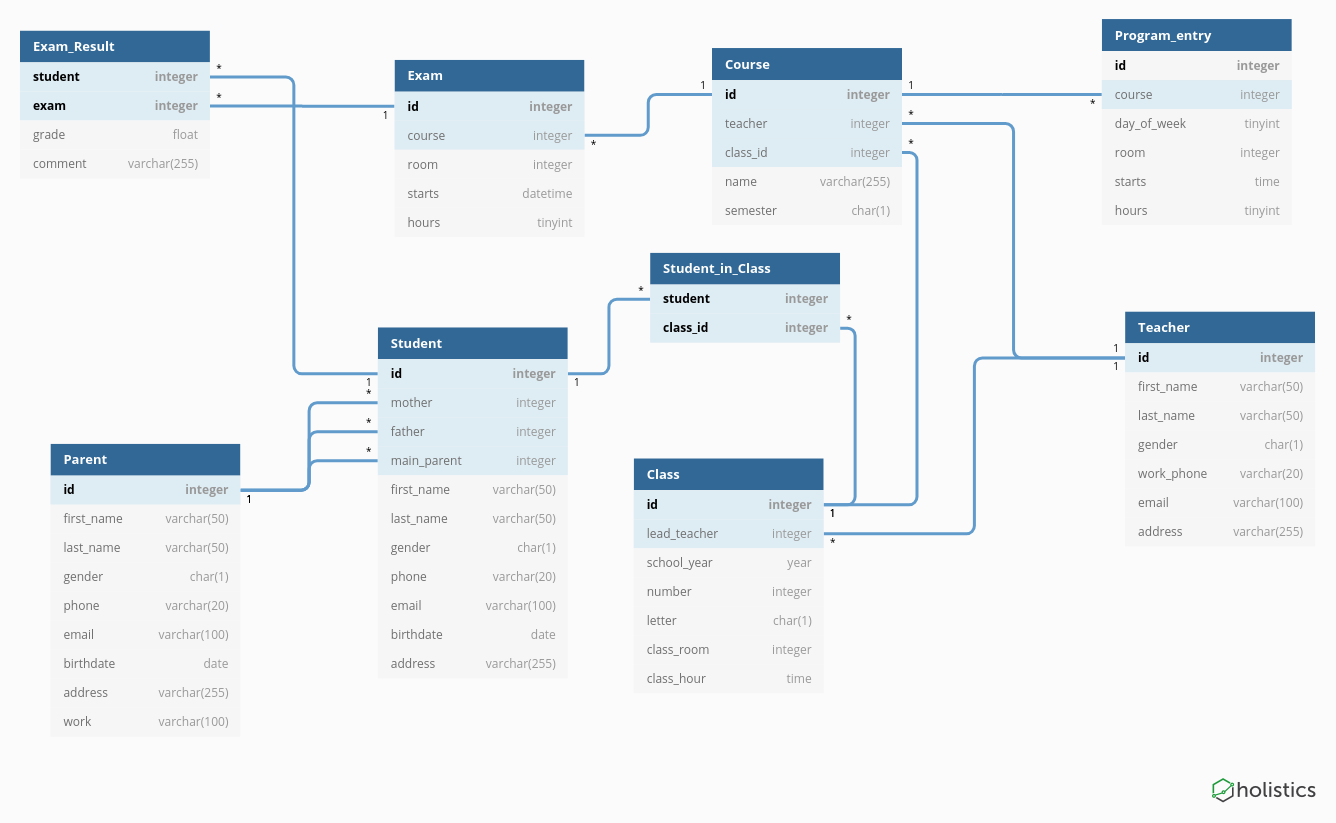
\includegraphics[width=\textwidth]{table_diagram}
\restoregeometry{}
\section{Описание на функциите}
\subsection{full\_gender}
Функията full\_gender по символ за пол връща пълното наименование на пола, ако той е 'M' или 'F',
иначе връща 'Other'.
\subsection{full\_semester}
Функията full\_semester по символ за срок връща пълното наименование на срока, ако той е 'F' или 'S',
иначе връща 'Unknown'.
\subsection{day\_of\_week\_as\_string}
Функията day\_of\_week\_as\_string по число за ден от седмицата връща пълното наименование на деня,
ако аргумента е валиден ден от седмицата (цяло число между 1 и 5 включително),
иначе връща 'Unknown'.
\section{Описание на тригерите}
\subsection{Before\_Insert\_Exam\_Result}
Тригера се грижи за налагане на ограничение върху
стойността на колоната grade - да бъде число в интервала [2.0, 3.0],
задействано преди добавяне в таблицата Exam\_Result.
\subsection{Before\_Update\_Exam\_Result}
Тригера се грижи за налагане на ограничение върху
стойността на колоната grade - да бъде число в интервала [2.0, 3.0],
задействано преди обновяне в таблицата Exam\_Result.
\subsection{Before\_Insert\_Course}
Тригера се грижи за налагане на ограничение върху
стойността на колоната semester - да бъде или 'F' или 'S',
задействано преди добавяне в таблицата Course.
\subsection{Before\_Update\_Course}
Тригера се грижи за налагане на ограничение върху
стойността на колоната semester - да бъде или 'F' или 'S',
задействано преди обновяне в таблицата Course.
\subsection{Before\_Insert\_Program\_entry}
Тригера се грижи за налагане на ограничение върху
стойността на колоната day\_of\_week - да бъде цяло число в списъка (1, 2, 3, 4 5),
задействано преди добавяне в таблицата Program\_entry.
\subsection{Before\_Update\_Program\_entry}
Тригера се грижи за налагане на ограничение върху
стойността на колоната day\_of\_week - да бъде цяло число в списъка (1, 2, 3, 4 5),
задействано преди обновяне в таблицата Program\_entry.
\section{Описание на изгледите}
\subsection{Grade}
Изгледа Grade предоставя пълна информация за една оценка.
Информацията се извлича от таблиците: Exam\_Result,
Student, Exam, Exam\_Result, Course, Class и Teacher.
Като колоните, до които дава достъп изгледа са:
Exam\_Result.student, Student.first\_name,
Student.last\_name, Class.id, Class.school\_year,
Class.number, Class.letter, Course.id, Course.name,
Course.semester, Teacher.id, Teacher.first\_name,
Teacher.last\_name, Exam.starts, Exam\_Result.grade \\
и Exam\_Result.comment.
\subsection{Program}
Изгледа Program предоставя пълна информация за един учебен час от програмата.
Информацията се извлича от таблиците: Program\_entry,
Course, Class и Teacher.
Като колоните, до които дава достъп изгледа са:
Program\_entry.id,
Program\_entry.day\_of\_week,
Program\_entry.room,
Program\_entry.starts, \\
Program\_entry.hours,
Program\_entry.course,
Course.name,
Course.semester,
Course.teacher,
Teacher.first\_name,
Teacher.last\_name,
Course.class\_id,
Class.school\_year,
Class.number,
Class.letter.
\section{Описание на приложението за достъп с резултатите от заявката}
Приложението за достъп е изключително просто (семпло).
Написано е на езика Java-Script и ползва пакета mqsql за свързване с mysql сървъра.
Приложението се свързва към сървъра посредством забита в кода информация
за потребител, парола и база, които всички са test-drive.
След, което чете подадения чрез командните параметри файл, който трябва да е валиден sql
скрипт, не съдържаш командни DELIMITER понеже, те не се поддържат от използвания пакет.
След свързване, то изпълнява заявките от скрипта и извежда резултат.
\subsection{Резултати при изпълнение с combined\_sql/test.sql}
Скрипта създава таблиците, попълва ги, след което съсдава изгледите и накрая прави заявка към всеки изглед.
Резултатите се подобни на тези, ако използване CLI-то на mysql.
\subsubsection{Създаване на таблица}
\begin{listing}
\begin{minted}[xleftmargin=21pt, tabsize=4]{js}
OkPacket {
    fieldCount: 0,
    affectedRows: 0,
    insertId: 0,
    serverStatus: 10,
    warningCount: 0,
    message: '',
    protocol41: true,
    changedRows: 0
}
\end{minted}
\end{listing}
\subsubsection{Вмъкване в таблица}
\begin{listing}
\begin{minted}[xleftmargin=21pt, tabsize=4]{js}
OkPacket {
    fieldCount: 0,
    affectedRows: 3,
    insertId: 0,
    serverStatus: 10,
    warningCount: 0,
    message: '&Records: 3  Duplicates: 0  Warnings: 0',
    protocol41: true,
    changedRows: 0
}
\end{minted}
\end{listing}
\subsubsection{Ред, резултат от заявка към Grade}
\begin{listing}
\begin{minted}[xleftmargin=21pt, tabsize=4]{js}
RowDataPacket {
    student: 3,
    student_first_name: 'Jordan',
    student_last_name: 'Angelov',
    class: 1,
    school_year: 2016,
    class_number: 12,
    class_letter: 'B',
    course: 1,
    course_name: 'Mathematics',
    course_semester: 'F',
    teacher: 1,
    teacher_first_name: 'Veselka',
    teacher_last_name: 'Hristova',
    exam_date: 2016-01-15T08:00:00.000Z,
    grade: 6,
    comment: null
}
\end{minted}
\end{listing}
\subsubsection{Ред, резултат от заявка към Program}
\begin{listing}
\begin{minted}[xleftmargin=21pt, tabsize=4]{js}
RowDataPacket {
    entry: 3,
    day_of_week: 3,
    room: 32,
    starts: '11:20:00',
    hours: 3,
    course: 5,
    subject: 'Technology of Programming',
    semester: 'F',
    teacher: 2,
    teacher_first_name: 'Kiril',
    teacher_last_name: 'Mitov',
    class_id: 1,
    school_year: 2016,
    class_number: 12,
    class_letter: 'B'
}
\end{minted}
\end{listing}
\end{document}